% Векторизация нахождения пересечения объемной и поверхностной сеток .
\subsection{Векторизация нахождения пересечения объемной и поверхностной сеток для микропроцессоров с поддержкой AVX-512}

\begin{figure}[ht]
	\centering
		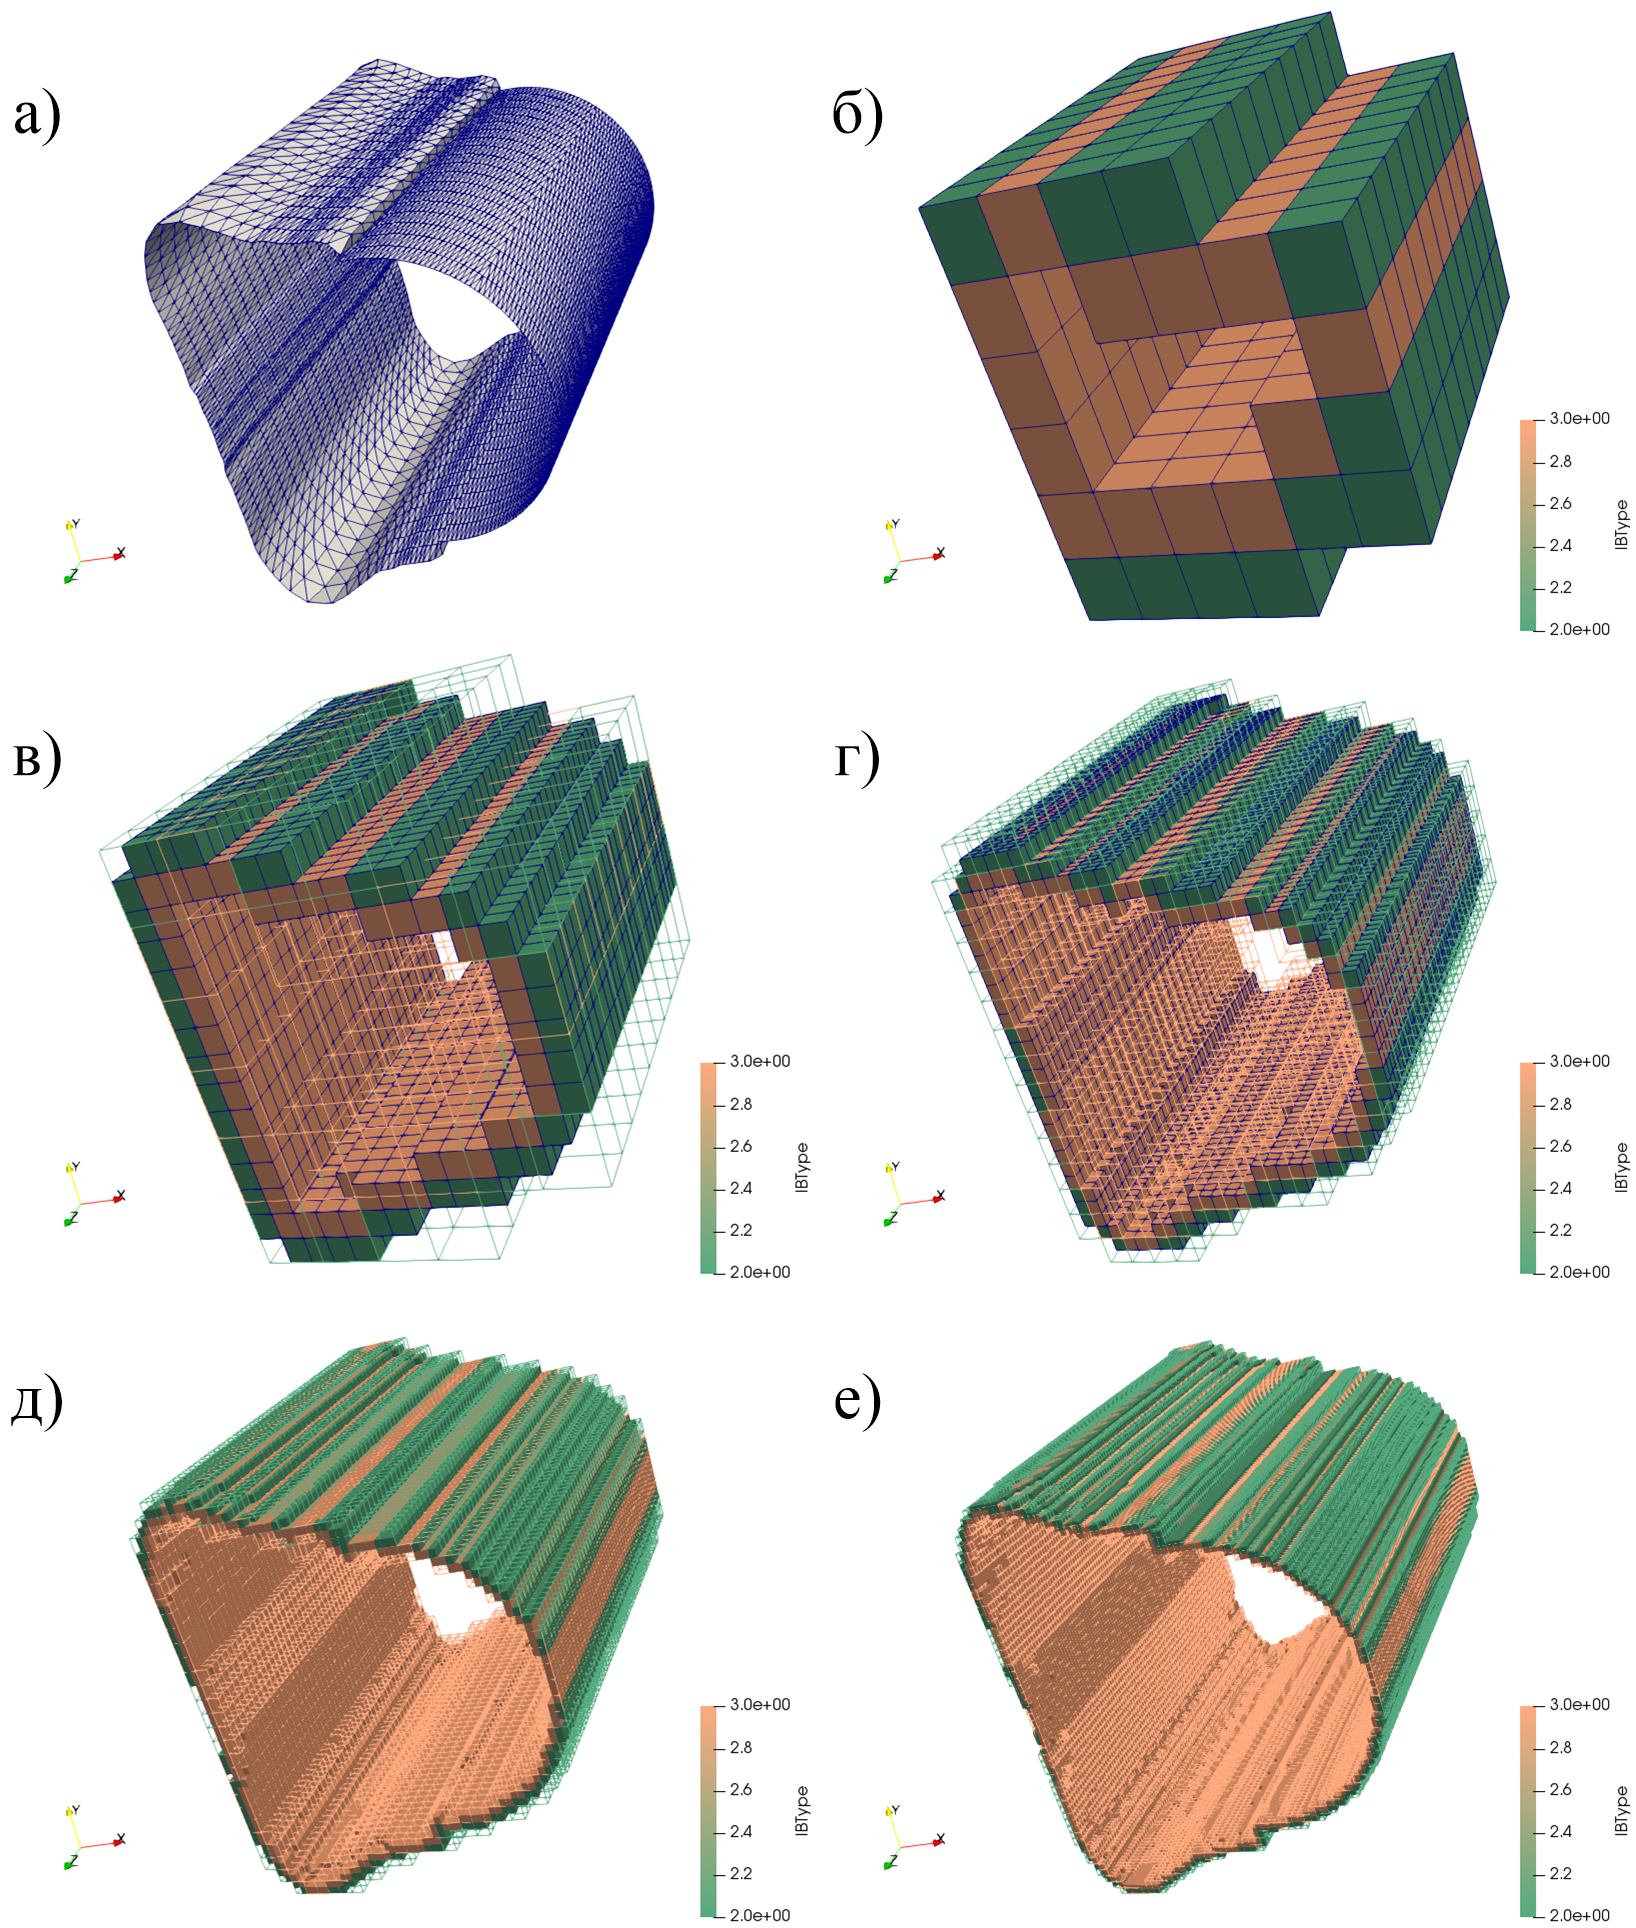
\includegraphics[width=0.5\textwidth]{./pics/text_4_mesh_intersect/contour.png}
	\caption{Иллюстрация пересечения поверхностной сетки и объемных сеток с разным количеством ячеек. На рисунках цветами обозначены только граничные и фиктивные ячейки объемной сетки (граничные -- зеленые, фиктивные -- бежевые). а) Исходная геометрия поверхностной сетки. б) Размер объемной сетки 10x10x10. в) Размер объемной сетки 25x25x25. г) Размер объемной сетки 50x50x50. д) Размер объемной сетки 100x100x100. е) Размер объемной сетки 150x150x150.}
	\label{fig:text_1_mesh_intersect_contour}
\end{figure}

\subsubsection{Оптимизация поиска пересечения сеток}

Ячейки объемной сетки являются прямоугольными параллелепипедами.
Ячейки поверхностной сетки являются треугольниками.
Для того, чтобы найти все ячейки объемной сетки, которые пересекаются с поверхностью, в общем случае необходимо проверить факт пересечения каждой объемной ячейки с каждой поверхностной ячейкой.
В общем случае данная процедура является очень затратной, так как сетки могут содержать большое количество ячеек.
Вместо этого для каждой ячейки поверхностной сетки сначала будем определять диапазон ячеек объемной сетки, с которыми в принципе возможно пересечение.

Пусть изначально объемная сетка, описывающая область [Xl, Xh]x[Yl, Yh]x[Zl, Zh], размера SxxSyxSz,  разделена на одинаковые базовые ячейки (которые впоследствии могут быть разделены на более мелкие) размера sx×sy×sz, где
\begin{equation}
	n_x = \frac{S_x}{s_x}, \ n_y = \frac{S_y}{s_y}, \ n_z = \frac{S_z}{s_z}
\end{equation}

(nx -- количество базовых ячеек по направлению x, аналогично для направлений y и z).
Таким образом, объемная сетка представлена трехмерным массивом базовых ячеек, координаты которых (xl, xh, yl, yh, zl, zh) могут быть вычислены по индексам (i, j, k) в данном трехмерном массиве:
\begin{equation}
	\begin{aligned}
		& x_l(i) = X_l + i s_x \\
		& x_h(i) = X_l + (i + 1) s_x \\
		& y_l(j) = Y_l + j s_y \\
		& y_h(j) = Y_l + (j + 1) s_y \\
		& z_l(k) = Z_l + k s_z \\
		& z_h(k) = Z_l + (k + 1) s_z		
	\end{aligned}
\end{equation}

Для треугольника, являющегося ячейкой поверхностной сетки, вершинами которого являются точки A(xA, yA, zA), B(xB, yB, zB), C(xC, yC, zC), можно найти охватывающий прямоугольный параллелепипед, координаты которого равны
\begin{equation}
	\begin{aligned}
		& \tilde{x}_l = min(x_A, x_B, x_C) \\
		& \tilde{x}_h = max(x_A, x_B, x_C) \\
		& \tilde{y}_l = min(y_A, y_B, y_C) \\
		& \tilde{y}_h = max(y_A, y_B, y_C) \\
		& \tilde{z}_l = min(z_A, z_B, z_C) \\
		& \tilde{z}_h = max(z_A, z_B, z_C)
	\end{aligned}
\end{equation}

Если треугольник пересекает некоторую объемную ячейку, то его охватывающий прямоугольный параллелепипед также пересекает эту ячейку.
То есть для определения пересечения поверхностной ячейки со всеми ячейками объемной сетки достаточно проверить только те ячейки, с которыми пересекается охватывающий прямоугольный параллелепипед рассматриваемого треугольника.
Так как координаты анализируемых параллелепипедов могут быть записаны явно, то можно вычислить диапазоны индексов базовых ячеек, которые требуется проверить на вопрос пересечения с треугольником.
Факт пересечения по координате x двух отрезков и можно записать в виде системы из двух неравенств
\begin{equation}
	\left\{
		\begin{aligned}
			x_l(i) \le \tilde{x}_h \\
			x_h(i) \ge \tilde{x}_l
		\end{aligned}
	\right.
\end{equation}

Преобразовав данную систему, а также выполнив аналогичные действия для координат по y и z, получим итоговые диапазоны индексов базовых ячеек
\begin{equation}
	\left\{
		\begin{aligned}
			\frac{\tilde{x}_l - X_l}{s_x} - 1 \le i \le \frac{\tilde{x}_h - X_l}{s_x} \\
			\frac{\tilde{y}_l - Y_l}{s_y} - 1 \le i \le \frac{\tilde{y}_h - Y_l}{s_y} \\
			\frac{\tilde{z}_l - Z_l}{s_z} - 1 \le i \le \frac{\tilde{z}_h - Z_l}{s_z}
		\end{aligned}
	\right.
\end{equation}

Данный диапазон индексов содержит малую долю всех ячеек объемной сетки.
В данном случае не требуется проводить анализ ускорения от этого преобразования, так как при его отсутствии поиск пересечения сеток просто нежизнеспособен.

Заметим, что при измельчении объемной сетки алгоритм поиска пересечения изменяется не сильно, так как диапазоны индексов базовых ячеек не меняются, однако кроме базовых ячеек обязательными для проверки становятся также все их дочерние ячейки.

\subsubsection{Векторизация вычислений}

Рассмотрим реализацию функции \texttt{tri\_box\_intersect(xa ya, za, xb, yb, zb, xc, yc, zc, xl, xh, yl, yh, zl, zh) -> int}, анализирующую наличие пересечения треугольника и прямоугольного параллелепипеда.
Функция возвращает 1, если пересечение есть, и 0, если пересечения нет.
Логика работы функции следующая.
Сначала коэффициенты системы неравенств (4) заносятся в двумерный массив коэффициентов b[bec][3], где bec (basic equations count) -- количество исходных неравенств системы (в нашем случае 9).
Затем выполняется один шаг свертывания системы с одновременным поиском множества решения для переменной $beta$.
Перед началом свертывания множество допустимых значений для переменной $beta$ принимается в виде отрезка [0, 1] (lo = 0, hi = 1).
По мере свертывания системы неравенств (4) происходит сокращение данного множеств решений.
Если на каком-то  этапе свертывания множество решений обращается в пустое (lo > hi), то функция заканчивает работу и возвращает 0.
Если после выполнения всех действий свертывания множество решений осталось ненулевым, то это означает наличие пересечения, и функция возвращает 1.
Реализация свертывания системы уравнений с помощью метода из [6] представлена на рис. 2.

\begin{figure}[ht]
	\centering
		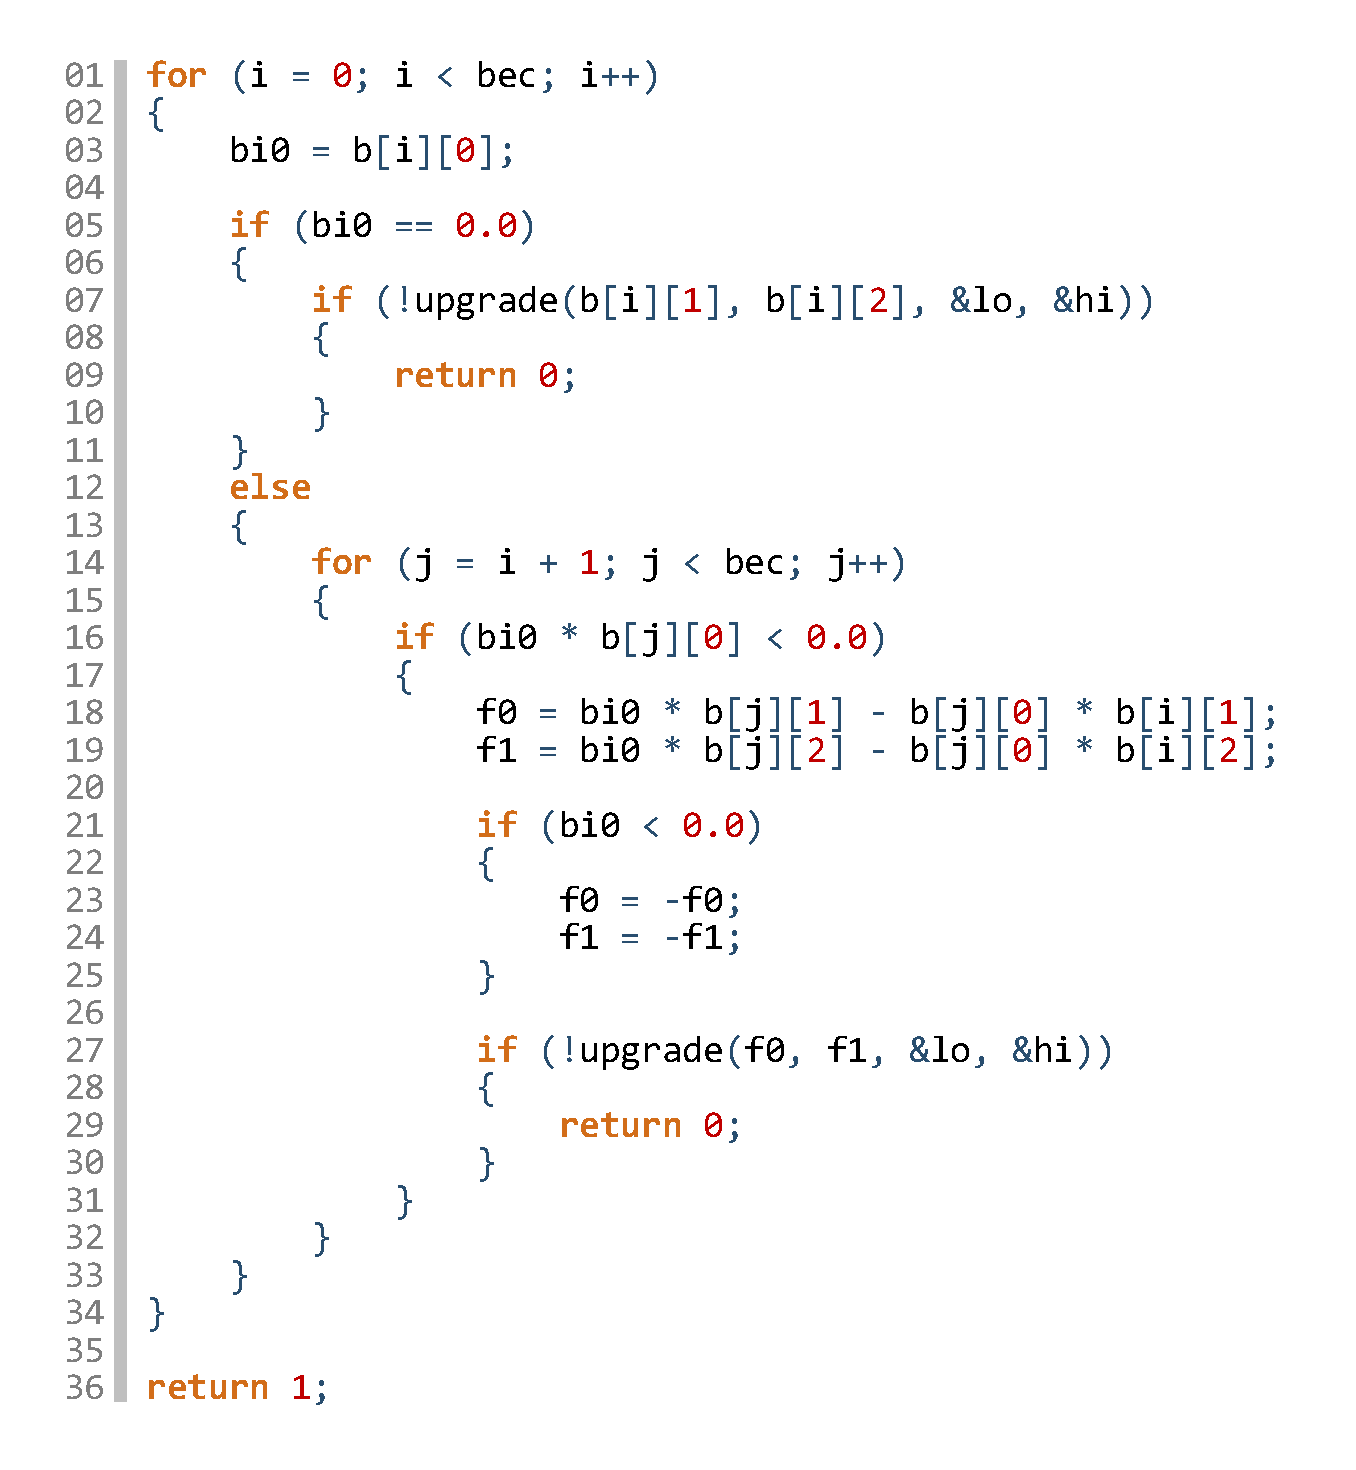
\includegraphics[width=0.6\textwidth]{./pics/text_4_mesh_intersect/pic_tri_intersect_orig.pdf}
	\caption{Исходная реализация свертывания системы линейных неравенств для определения пересечения треугольника и прямоугольного параллелепипеда.}
	\label{fig:text_1_mesh_intersect_tri}
\end{figure}

Получившийся код можно охарактеризовать как имеющий сложное управление, уровень вложенности конструкций в нем достигает 5 (for-if-for-if-if), к тому же участок содержит 3 выхода из функции.
Функция upgrade, которая вызывается из кода на рис. 2, предназначена для обновления текущего множества допустимых значений для переменной $\beta$ с учетом нового полученного ограничения вида  , коэффициенты которого передаются в первом и втором параметрах.
Текущее множество решений является отрезком с границами, хранящимися в переменных lo и hi, и в зависимости от знака коэффициента   одна из этих границ внутри вызова функции upgrade может измениться (граница lo может увеличиться, либо граница hi может уменьшиться).
Если после обновления множества решений оно оказывается пустым (нижняя граница становится больше верхней), то функция upgrade возвращает 0, в противном случае она возвращает 1.

После рассмотрения реализации функции \texttt{tri\_box\_intersect} можно перейти к векторизации вычислений.
Для анализа пересечения двух сеток необходимо вызывать функцию \texttt{tri\_box\_intersect} многократно с разными наборами входных параметров.
Для оптимизации этого процесса реализуем функцию \texttt{tri\_box\_intersect\_16}, объединяющую внутри себя обработку 16 вызовов функции \texttt{tri\_box\_intersect} (используется объединение 16 вызовов, так как это совпадает с количеством элементов вещественных данных одинарной точности в одном векторе \texttt{\_\_m512}, \texttt{VEC\_WIDTH = 16}).
В первом приближении реализация функции \texttt{tri\_box\_intersect\_16} представлена на рис. 3. Конечно в реальной задаче требуется обрабатывать миллионы вызовов, однако они могут быть разбиты на группы по 16 и обработаны с помощью функции \texttt{tri\_box\_intersect\_16}, поэтому остановимся подробнее на векторизации данной функции.

\begin{figure}[ht]
	\centering
		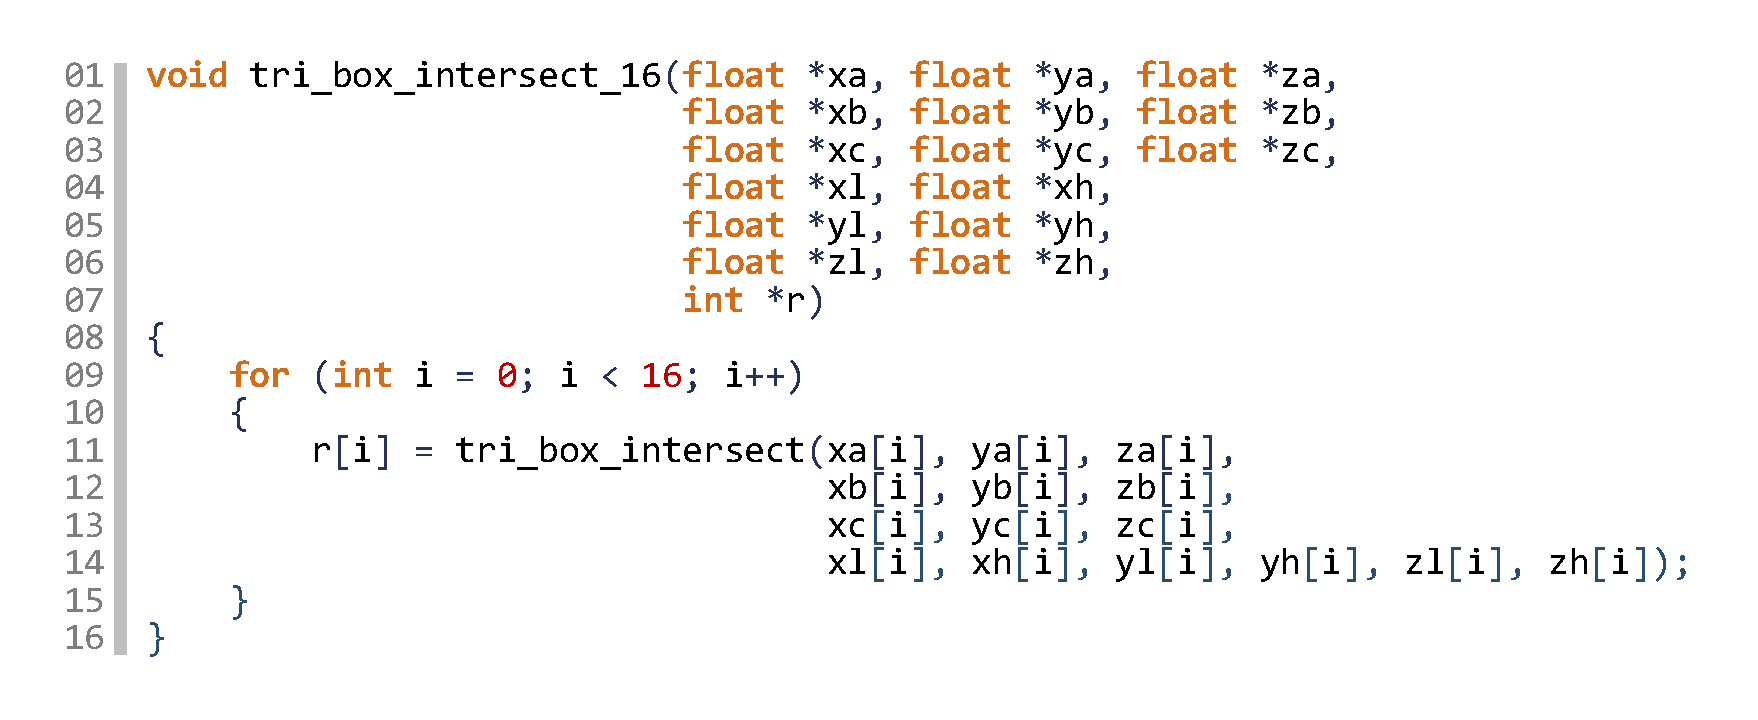
\includegraphics[width=1.0\textwidth]{./pics/text_4_mesh_intersect/pic_tri_intersect_16_orig.pdf}
	\caption{Исходная реализация функции, объединяющей 16 вызовов функции \texttt{tri\_box\_intersect}.}
	\label{fig:text_1_mesh_intersect_tri16}
\end{figure}

Для векторизации функции \texttt{tri\_box\_intersect\_16} следует выполнить подстановку тела функции \texttt{tri\_box\_intersect} в место ее вызова.
После выполнения данного преобразования получаем программный контекст, содержащий сложное управление и в частности гнездо из трех вложенных циклов, не считая условий.
Данный контекст не может быть векторизован компилятором автоматически, поэтому будем проводить его векторизацию в ручном режиме с использованием функций-интринсиков, которые позволяют напрямую использовать инструкции AVX-512 в синтаксисе языка программирования C без использования ассемблера.

Заметим, что между итерациями внешнего цикла (рис. 3, строка 09) отсутствуют зависимости, то есть цикл является плоским, и его итерации могут быть выполнены в любом порядке, в том числе и одновременно.
Такие циклы поддаются векторизации путем перевода тела в предикатное представление и заменой скалярных инструкций на векторные.
Наиболее тонким местом при векторизации тела плоского цикла являются условия, то есть наличие конструкций if-else [21].
Альтернативные ветви таких конструкций должны быть объединены в предикатном коде под противоположными предикатами.
Наличие большого количества условных операторов в исходном коде порождает множество инструкций под нулевыми предикатами в результирующем коде, что негативно сказывается на производительности.
Для уменьшения количества условных операторов, можно использовать математические тождества, заменяющие условные конструкции на команды, имеющие векторные аналоги в наборе инструкций AVX-512.
Для данных целей хорошо подходят такие векторные команды как abs, min, max, blend, avg и другие.
Например в рассматриваемом коде вычисление значений f0 и f1 в строках 18-25 на рис. 2 с учетом условия b[i][0] * b[j][0] < 0 может быть заменено на следующее:

\begin{lstlisting}[caption={caption},label={label}]
f0 = fabs(bi0) * b[j][1]
     + fabs(b[j][0]) * b[i][1]
f1 = fabs(bi0) * b[j][2]
     + fabs(b[j][0]) * b[i][2]
\end{lstlisting}

Похожие трудности вызывает условие if в строке 05 на рис 2. Данное условие имеет альтернативную ветку, содержащую цикл.
Слияние данных двух ветвей снижает производительность результирующего кода, поэтому в данном случае выгодно применить расщепление внешнего цикла по конструкции if-else (в [22] данное преобразование фигурирует под названием loop distribution).
При этом образуются два гнезда циклов, каждое из которых может быть векторизовано независимо.
Заметим, что описанное преобразование в общем смысле не является эквивалентным, так как обе ветки условия if-else, а значит и тела образовавшихся циклов содержат выходы из функции, выполнение расщепления цикла может изменить условие, провоцирующее выход из функции.
По этой причине компилятор не способен выполнить данное преобразование автоматически.
Однако с точки зрения результата функции данное преобразование корректно, поэтому мы его и применяем.

Отметим еще один крайне положительный момент в рассматриваемом программном контексте.
Условием выхода из вложенных циклов является достижение индуктивной переменной значения bec.
Данное значение является константой, а значит не зависит от номера итерации, поэтому в векторный код это условие может быть перенесено без изменений.
В случае зависимости условия выхода из цикла от номера итерации само условие должно быть также векторизовано, что может привести к потерям производительности, причины которых описаны в [23] на примере векторизации сортировки Шелла.
Однако в рассматриваемом коде проблем векторизации циклов с нерегулярным количеством итераций нет.
На рис. 4 приведен получившийся предикатный код для функции \texttt{tri\_box\_intersect\_16}, а также схематично показана его транформации в векторный аналог.

\begin{figure}[ht]
	\centering
		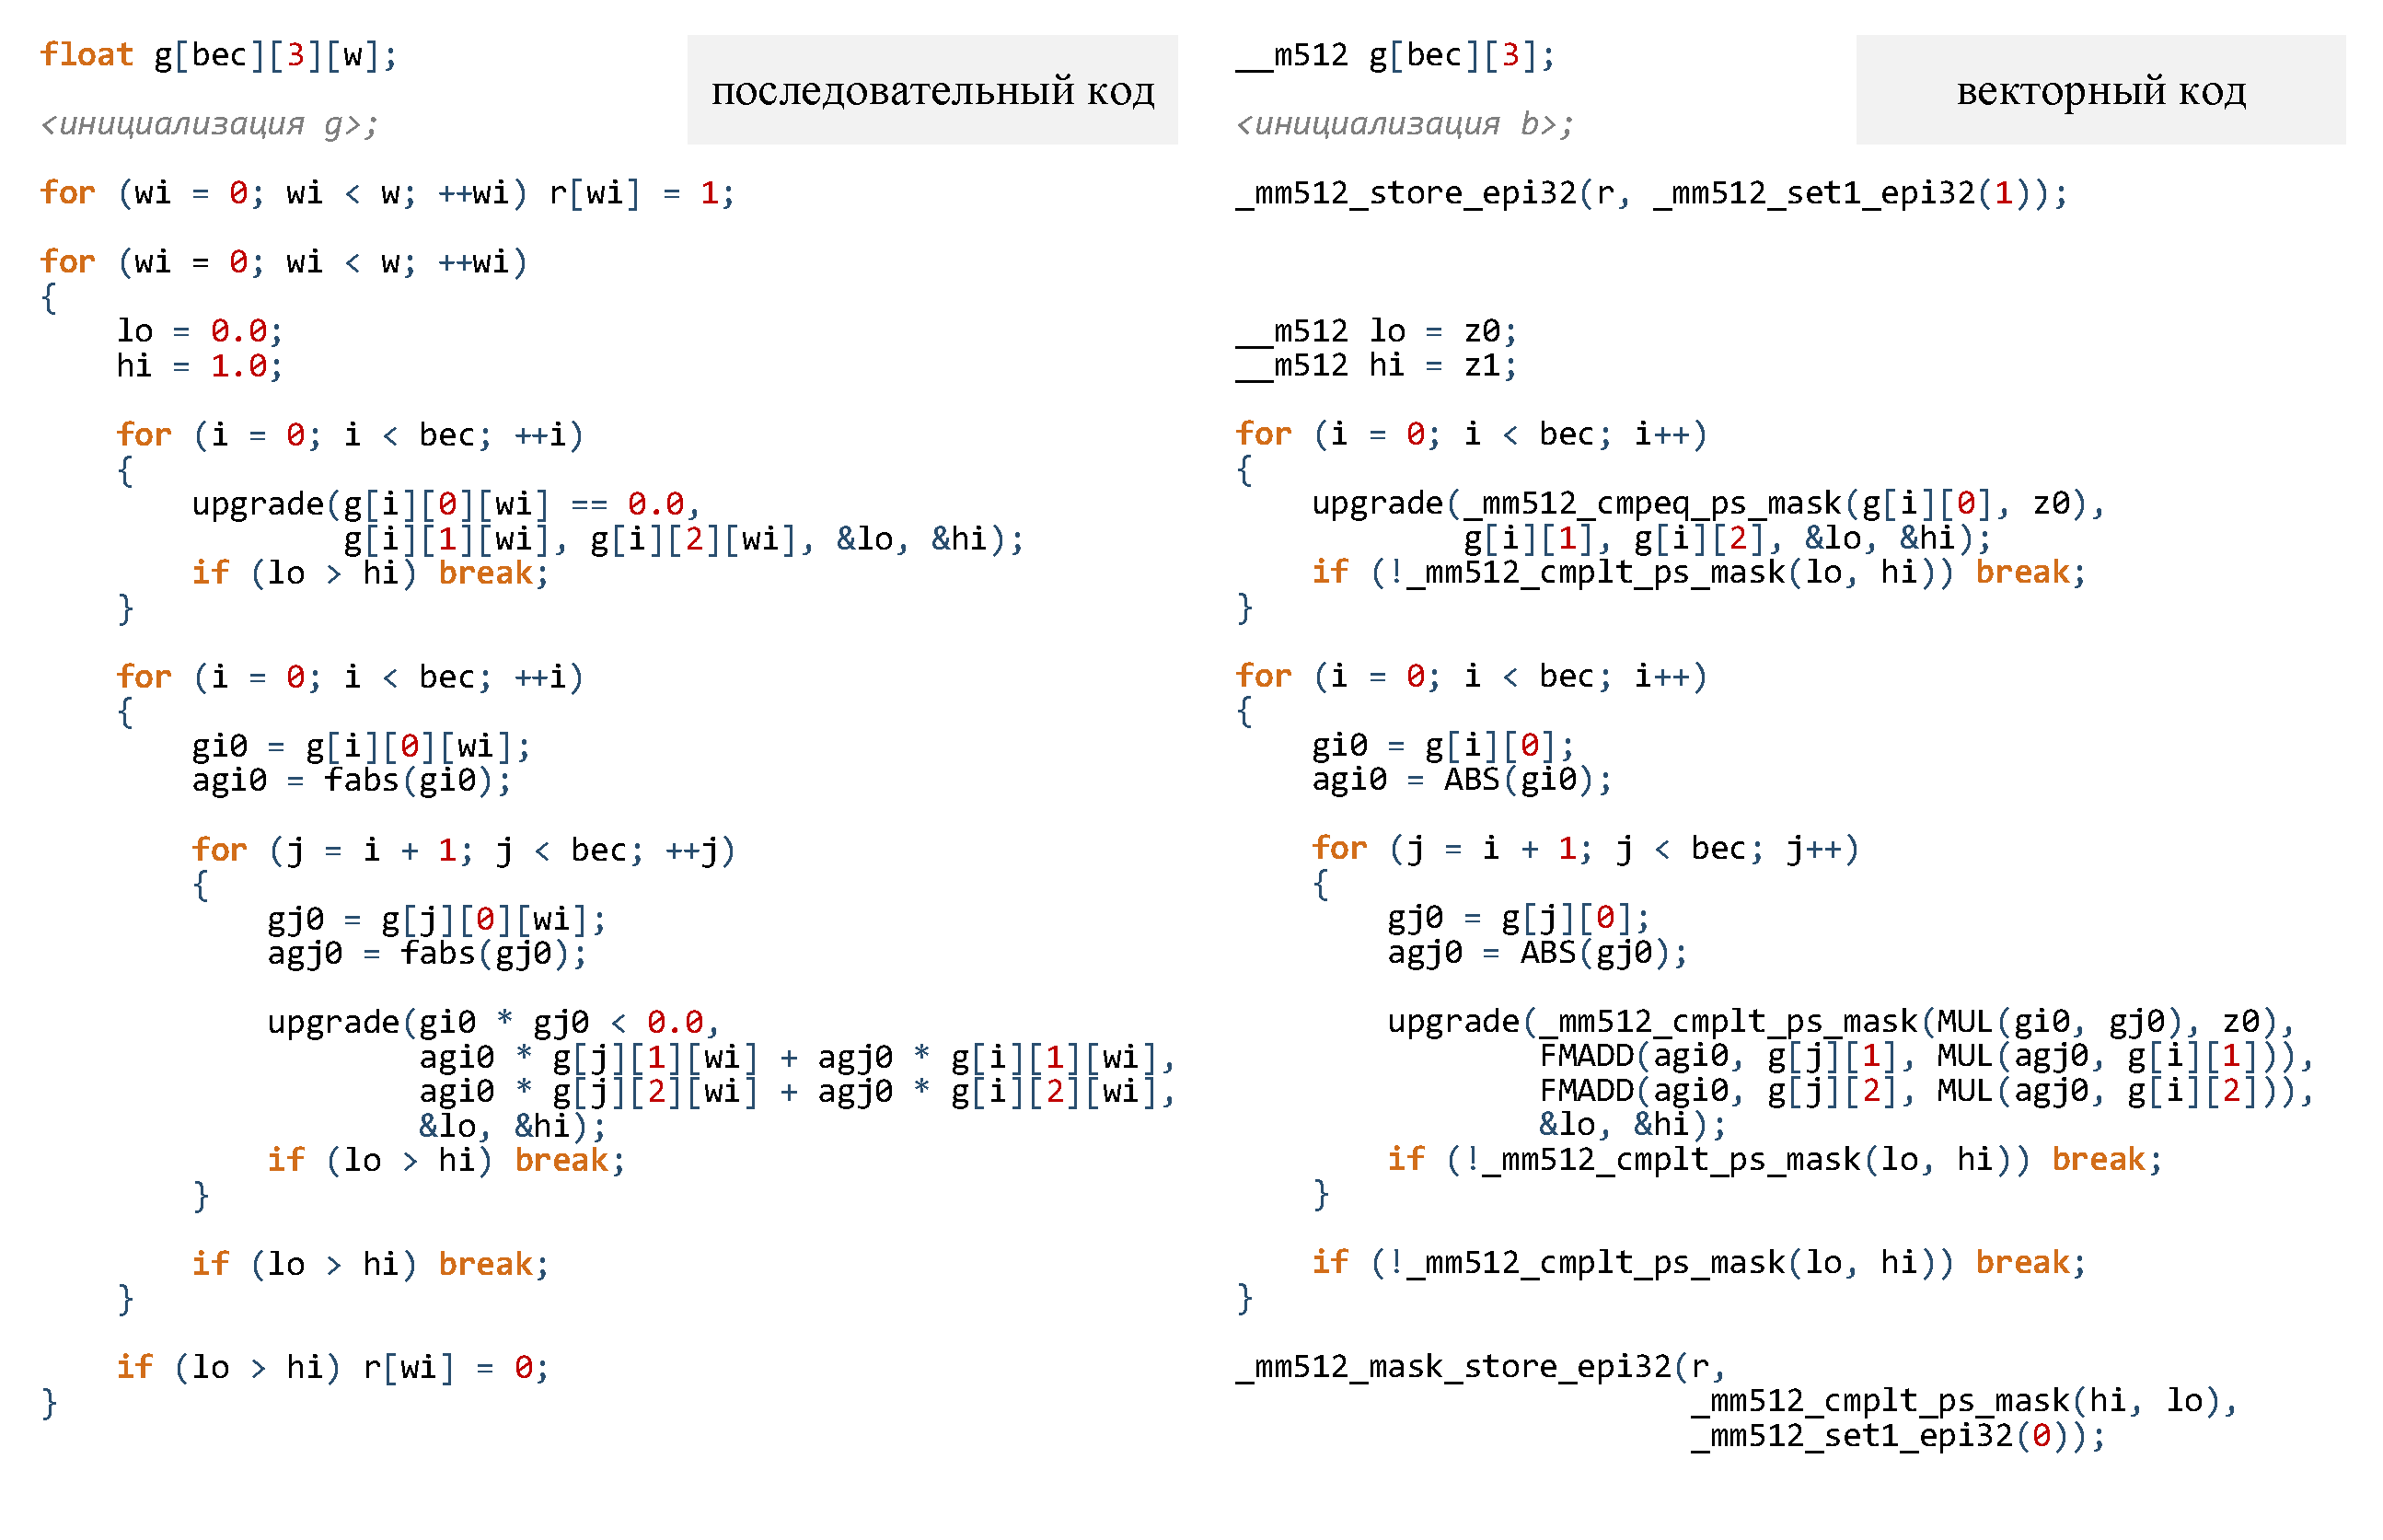
\includegraphics[width=1.0\textwidth]{./pics/text_4_mesh_intersect/final_scheme.pdf}
	\caption{Схема перевода последовательного кода в векторный аналог для ядра функции \texttt{tri\_box\_intersect\_16}}
	\label{fig:text_1_mesh_intersect_scheme}
\end{figure}

Из рис. 4 видно, что правильно составленный предикатный код (на рисунке слева) может быть довольно просто переведен в векторный аналог.
Для этого должны соблюдаться некоторые простые требования. Во-первых, необходимо удалить все else ветки в условных операторах.
Этого можно добиться, например, путем расщепления оператора if-else на два противоположных условия.
После этого любое условие if легко трансформируется в предикат на весь блок кода, находящийся под условием.
Во-вторых, вызовы функции не должны находиться под предикатами.
Вместо этого в нашем случае скалярное условие вызова функции upgrade трансформировалось в аргумент данной функции, и после этого код легко поддается векторизации.
В остальном все вещественные скалярные инструкции были просто заменены на векторные аналоги.
Также была выполнена векторизация функции upgrade с помощью слияния всех веток выполнения под их предикатами, результирующий код данной функции представлен на рис. 5.

\begin{figure}[ht]
	\centering
		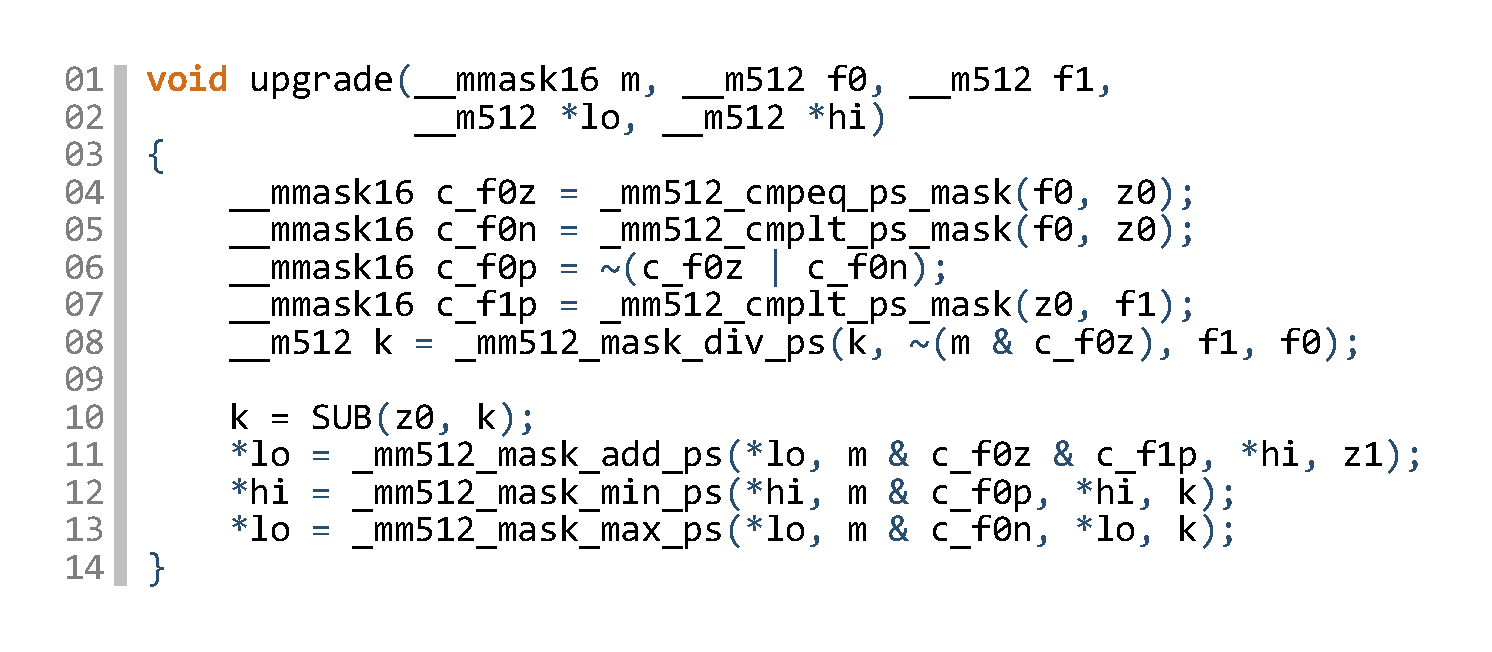
\includegraphics[width=0.6\textwidth]{./pics/text_4_mesh_intersect/upgrade_vec.pdf}
	\caption{Векторная реализация функции upgrade с пропагированным условием вызова внутрь функции}
	\label{fig:text_1_mesh_intersect_upgrade}
\end{figure}

В работе был выполнен анализ задачи об определении пересечения объемной декартовой сетки и поверхностной неструктурированной сетки, состоящей из треугольников.
Эффективное решение данной задачи напрямую влияет на производительность расчетных кодов обтекания тел со сложной и изменяющейся геометрией.
Была сформулирована математическая постановка задачи, предложены пути оптимизации ее реализации и выполнен анализ векторизации кода для микропроцессоров с поддержкой набора инструкций AVX-512.
В результате оптимизации была реализована векторная функция определения попарного пересечения 16 треугольников и 16 прямоугольных параллелепипедов.
Полученные программные коды были протестированы на суперкомпьютере МВС-10П, находящемся в МСЦ РАН, на сегменте, оборудованном микропроцессорами Intel Xeon Phi 7290 Knights Landing.
Векторизованный программный код продемонстрировал ускорение 6,7 раз по сравнению со скалярной версией, скомпилированной компилятором icc с полным набором оптимизаций.
Полученные результаты подтверждают пригодность описанного подхода к векторизации программного кода.
